\chapter{Results}\label{sec:results}

\section{13 TeV Results}

Figure\,\ref{fig:SignalRegionPlot_a} shows the background predictions as well as the observed $m(\tau_{1},\tau_{2},\MET)$ spectrum, in log scale, for the four 
channels considered in this analysis note: \mutau (top left), \ditauhad (top right), \etau (bottom left), \emu (bottom right). 
Table ~\ref{table:EvtSR_allMass} lists the number of estimated background events compared with the total number of observed events in data for each final state
considering the whole mass spectrum, while Table ~\ref{table:EvtSR_hiMass} lists those considering $M(\tau_1,\tau_2,\MET) >$ 300 GeV.
%Figure\,\ref{fig:SignalRegionPlot_b} shows the same unblinded result, except in normal scale in order to emphasize the low mass region. 
%(\textbf{placeholder text:} we are still blinded). 
The observed $m(\tau_{1},\tau_{2},\MET)$ spectrum in the signal region does not reveal any evidence for $Z^{\prime}\to\tau\tau$ production 
%(\textbf{this sentence and what follows is just placeholder text since we have not unblinded}). 
%The total predicted background rate is $19.8 \pm 4.2$, with QCD multijet,
%$t\bar{t}$, and $Z\to\tau\tau$ composing $\sim$ 76.3\%, 6.6\%, and 12.6\% of the rate respectively (see Table~\ref{table:expectations}).
%The distribution from the $m(W_{R})=2700$ GeV signal hypothesis is plotted with the background prediction in Figure\,\ref{fig:SignalRegionPlot} to illustrate how
%a hypothetical signal would appear above the SM background prediction. 
\begin{table}[ht]

\begin{center}
%\begin{subtable}
\begin{tabular}{| c | c | c | c | c | c |}
\hline
Process    & $\tau_h \tau_h$ & \mutau & \etau & \emu & \\
\hline
Drell-Yan  & 8    $\pm$ 3    & 882    $\pm$ 127   & 375    $\pm$ 118   & 321   $\pm$ 99    & \\
W+jets     & 0.1  $\pm$ 0.1  & 916    $\pm$ 96    & 546    $\pm$ 86    & 19    $\pm$ 11    & \\
Diboson    & 0.5  $\pm$ 0.5  & 29     $\pm$ 7     & 18.0   $\pm$ 4     & 108   $\pm$ 17    & \\
$t\bar{t}$ & --              & 26     $\pm$ 7     & 26     $\pm$ 8     & 223   $\pm$ 45    & \\
Multijet   & 49   $\pm$ 13   & 122    $\pm$ 84    & 117    $\pm$ 72    & 32    $\pm$ 24    & \\
\hline
Total      & 58   $\pm$ 13   & 1976   $\pm$ 180   & 1082   $\pm$ 162   & 703   $\pm$ 113   & \\
\hline     
Observed   & 55              & 1807               & 1113               & 728               & \\
\hline
\end{tabular}

\caption{Number of observed events in data and estimated background events for the whole mass range.
The uncertainties quoted on the number of background events represent the combined statistical and systematic uncertainty.
}
%\end{subtable}
\end{center}
\label{table:EvtSR_allMass}

\end{table}
%\begin{subtable}



\begin{table}
\begin{center}
\begin{tabular}{| c | c | c | c | c | c |}
\hline
Process    & $\tau_h \tau_h$ & \mutau & \etau & \emu & \\
\hline
Drell-Yan  & 5     $\pm$ 2      & 16 $\pm$ 4  & 9  $\pm$ 3 & 4  $\pm$ 2  & \\
W+jets     & 0.004 $\pm$ 0.004  & 23 $\pm$ 9  & 17 $\pm$ 7 & 1  $\pm$ 1  & \\
Diboson    & 0.02  $\pm$ 0.02   & 6  $\pm$ 3  & 2  $\pm$ 1 & 23 $\pm$ 4  & \\
$t\bar{t}$ & --                 & 4  $\pm$ 2  & 5  $\pm$ 1 & 65 $\pm$ 13 & \\
Multijet   & 18    $\pm$ 6      & 4  $\pm$ 3  & 6  $\pm$ 2 & 1  $\pm$ 1  & \\
\hline
Total      & 23    $\pm$ 6      & 51 $\pm$ 11 & 39 $\pm$ 8 & 94 $\pm$ 14 & \\
\hline     
Observed   & 20                & 42              & 40             & 96              & \\
\hline
\end{tabular}
%\end{subtable}
\caption{Number of observed events in data and estimated background events
in the region $M(\tau_{1},\tau_{2},\MET) >$ 300 GeV.
The uncertainties quoted on the number of background events represent the combined statistical and systematic uncertainty.
}
\end{center}
\label{table:EvtSR_hiMass}
\end{table}

An upper bound at 95\% confidence level (CL) is set on $\sigma \cdot BR$, 
where $\sigma$ is the cross-section for pair production of $pp\to Z^{\prime}$ and $BR$ the branching fraction for $Z^{\prime}\to\tau\tau$.

The calculation of the exclusion limit is obtained by using each bin of the $m(\tau_{1},\tau_{1},\MET)$ distribution to construct one bin of the likelihood 
and computing the 95\% confidence level (CL) upper limit on the signal cross-section using the asymptotic CL$_{s}$ method. 
%in the official limit calculation tool ``combine". 
Said differently, a shape based analysis is performed, using the $m(\tau_{1},\tau_{1},\MET)$ distribution as the fit discriminant to determine the 
likelihood of observing signal in the presence of the predicted background rate, given the observed yield in data. Systematic uncertainties are represented by nuisance parameters, which are profiled, assuming a log normal prior for normalization parameters, and Gaussian priors for mass-spectrum shape uncertainties.

The above procedure is performed using the Higgs limit calculation tool ``combine". The tool takes as input data cards with the yields and nuisance parameters in 
each $m(\tau_{1},\tau_{1},\MET)$ bin of the search channels. These data cards are provided by the four channels being considered, and the only further input that 
is required is the correlations within and across channels. As only an example, if all the channels had 10 bins from $0 < m(\tau_{1},\tau_{1},\MET) < 5000$ GeV 
(500 GeV/bin), this means there will be 10 cards per channel and therefore 40 cards in total for the four channels (if all the channels have the same bin size).
The cards corresponding to a specific final state, e.g. $\mu\tau_{h}$, were then combined using the ``CombineCards.py" tool provided by the Higgs limit tool, 
resulting in a single \textit{combined} data card. This procedure was performed for all the final states considered in the analysis, resulting in 
X \textit{combined} cards. The individual limits, per channel, were obtained by running the combine tool over each \textit{combined} card separately. The final 
combined limit was obtained by combining the four resulting \textit{combined} cards per channel described above, using the ``CombineCards.py" tool. In order to 
handle correlations within and across channels, the following approach was used. Each nuisance parameter was defined with a convention of two indices: the first 
index, $i$, denoted the channel ($i=\mu\tau_{h}=0$, $i=\tau_{h}\tau_{h}=1$, $i=$e$\tau_{h}=2$, $i=$e$\mu=3$) and the second one the type of process 
($j=$Signal$=0$, $j=$W+jets$=1$, etc.). Since the limit tool handles nuisance parameters with the same name as fully correlated, correlations across channels and 
processes were specified by utilizing the same $i$ and process index $j$, respectively.

Figure\,\ref{fig:Limits} shows the expected limits as well as the theoretical cross-section as functions of $m(Z^{\prime})$ mass for each channel. 
Figure\,\ref{fig:CombinedLimits} show the combined limit. A k factor of 1.3 has been used to scale the leading order (LO) signal cross-section. 
We exclude $Z^{\prime}$ (decaying through $Z^{\prime}\to\tau\tau$) masses below approximately 2.0 TeV. 

\begin{figure}[tbh!]
  \centering
%    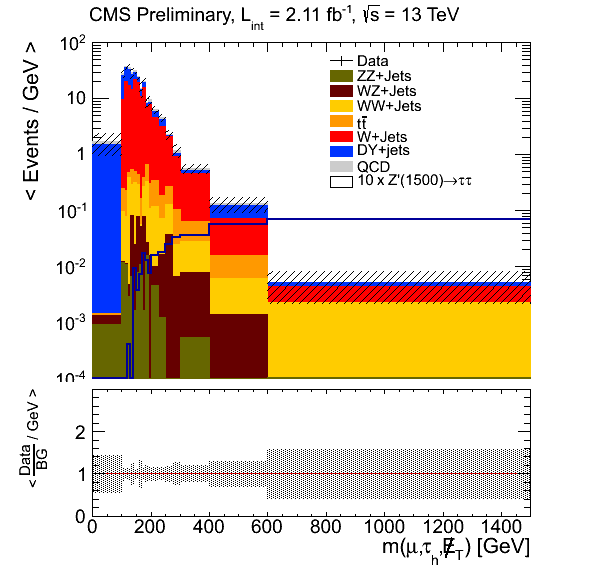
\includegraphics[width=0.4\textwidth]{figures/SRplot_NoData.png}
%    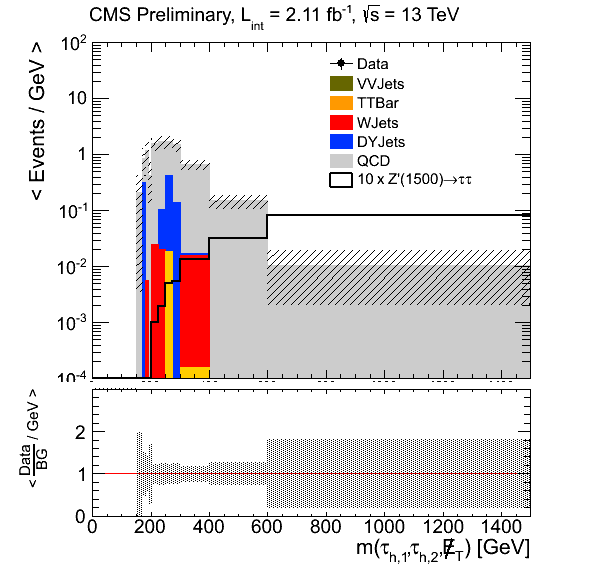
\includegraphics[width=0.4\textwidth]{figures/SRplot_diTauHad_NoData.png} \\
%   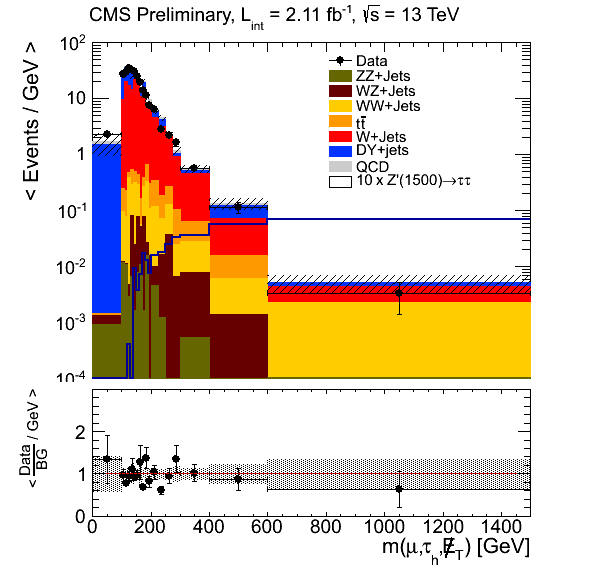
\includegraphics[width=0.4\textwidth]{figures/SR_muTau_Unblinded_LogScale_NewBinScheme_withoutPoissonErrorOnBGRateinBand.png}
%   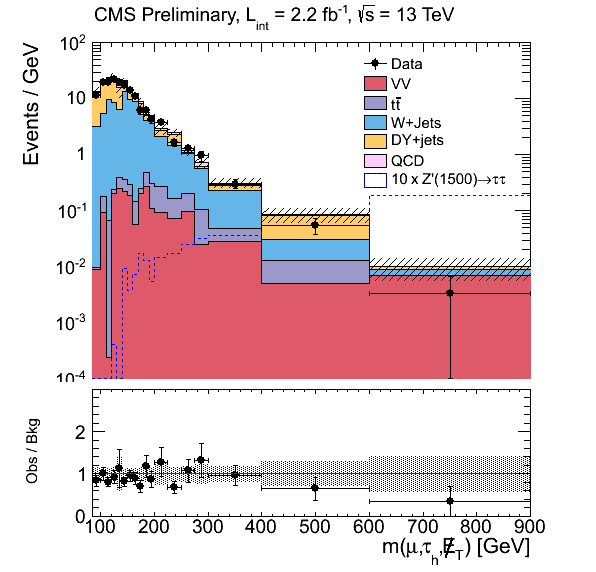
\includegraphics[width=0.4\textwidth]{figures/SR_muTau_Unblinded_LogScale_NewBinScheme_withoutPoissonErrorOnBGRateinBand_TightTo5WJetsIsoSideband_1or3Prong_ZaixingColors.png}
   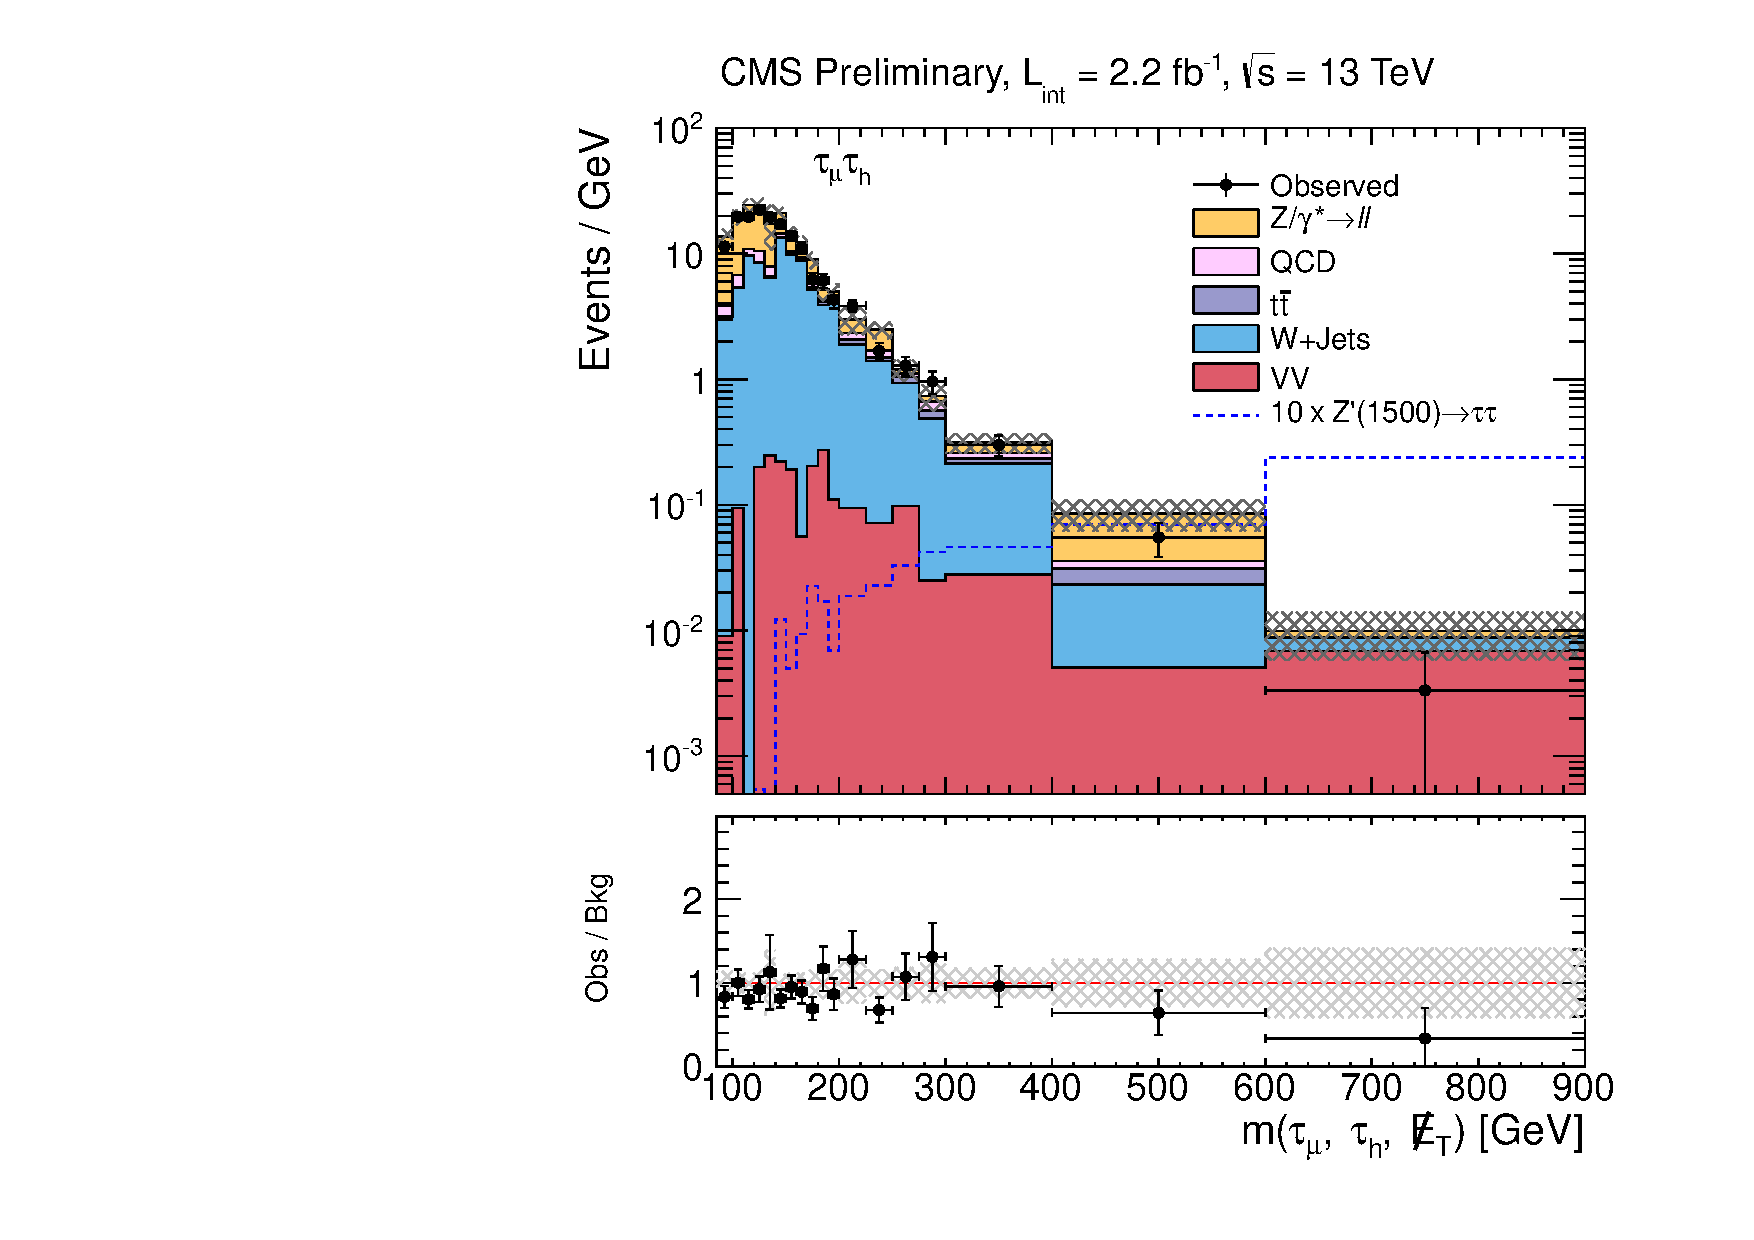
\includegraphics[width=0.4\textwidth]{figures/SR_muTau_Unblinded_LogScale_NewBinScheme_withoutPoissonErrorOnBGRateinBand_TightTo5WJetsIsoSideband_1or3Prong_ZaixingColors.pdf}
%   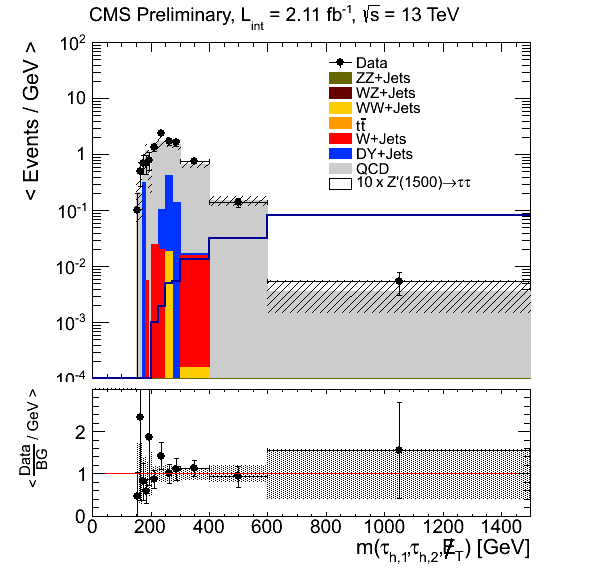
\includegraphics[width=0.4\textwidth]{figures/SR_diTauHad_Unblinded_LogScale_withoutPoissonErrorOnBGRateInBand.png} \\
%   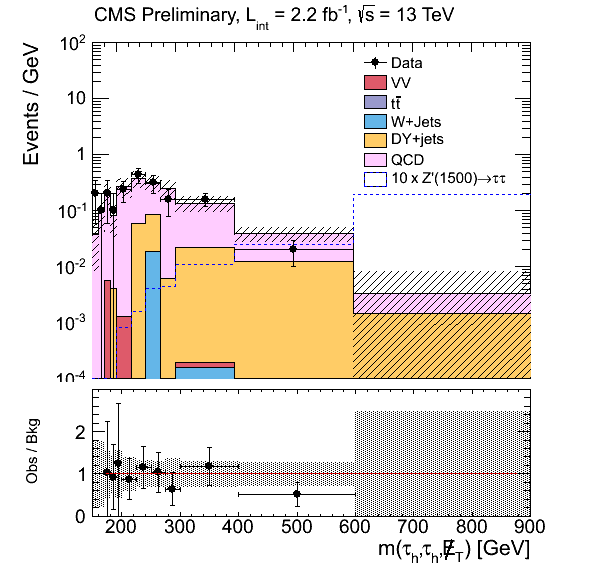
\includegraphics[width=0.4\textwidth]{figures/SR_diTauHad_Unblinded_LogScale_withoutPoissonErrorOnBGRateInBand_1or3prong_ZaixingColors.png} \\
   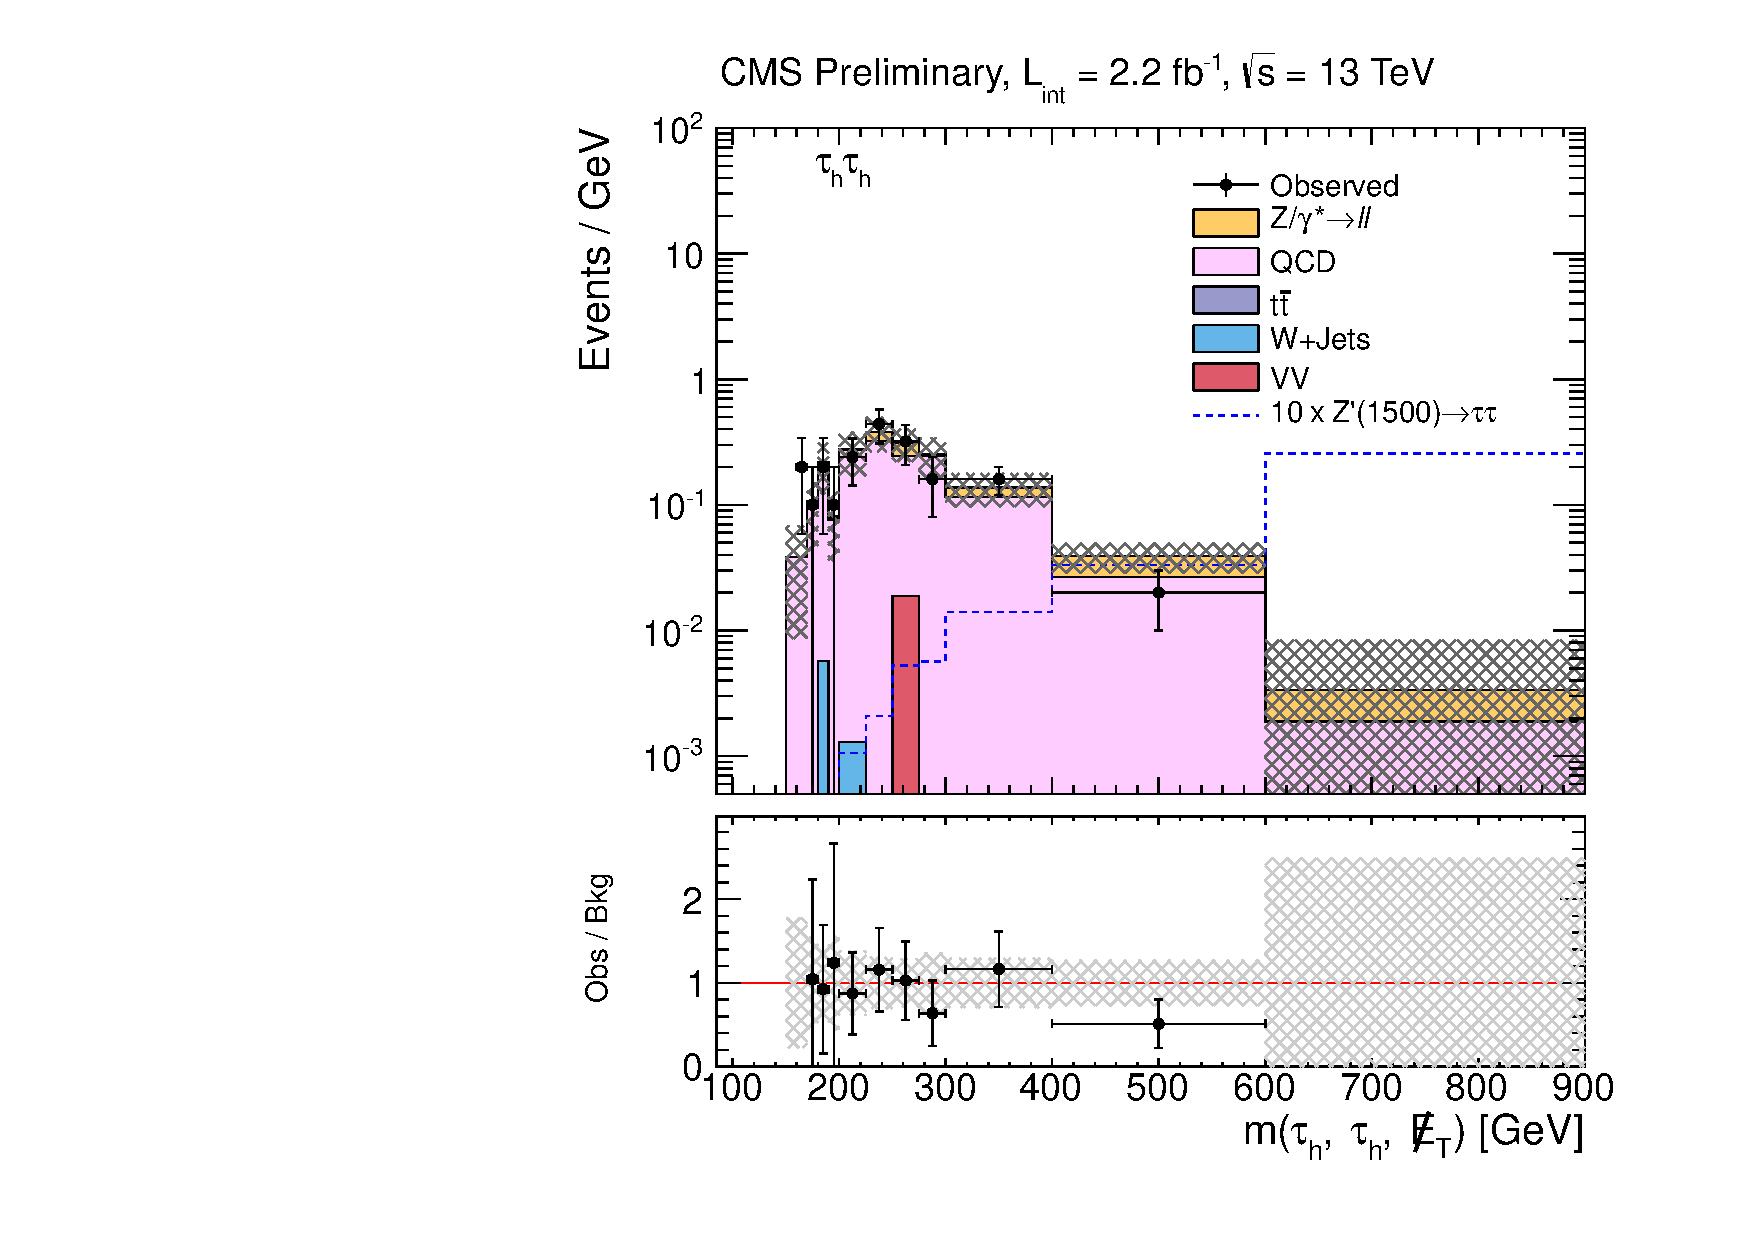
\includegraphics[width=0.4\textwidth]{figures/SR_diTauHad_Unblinded_LogScale_withoutPoissonErrorOnBGRateInBand_1or3prong_ZaixingColors.pdf} \\
   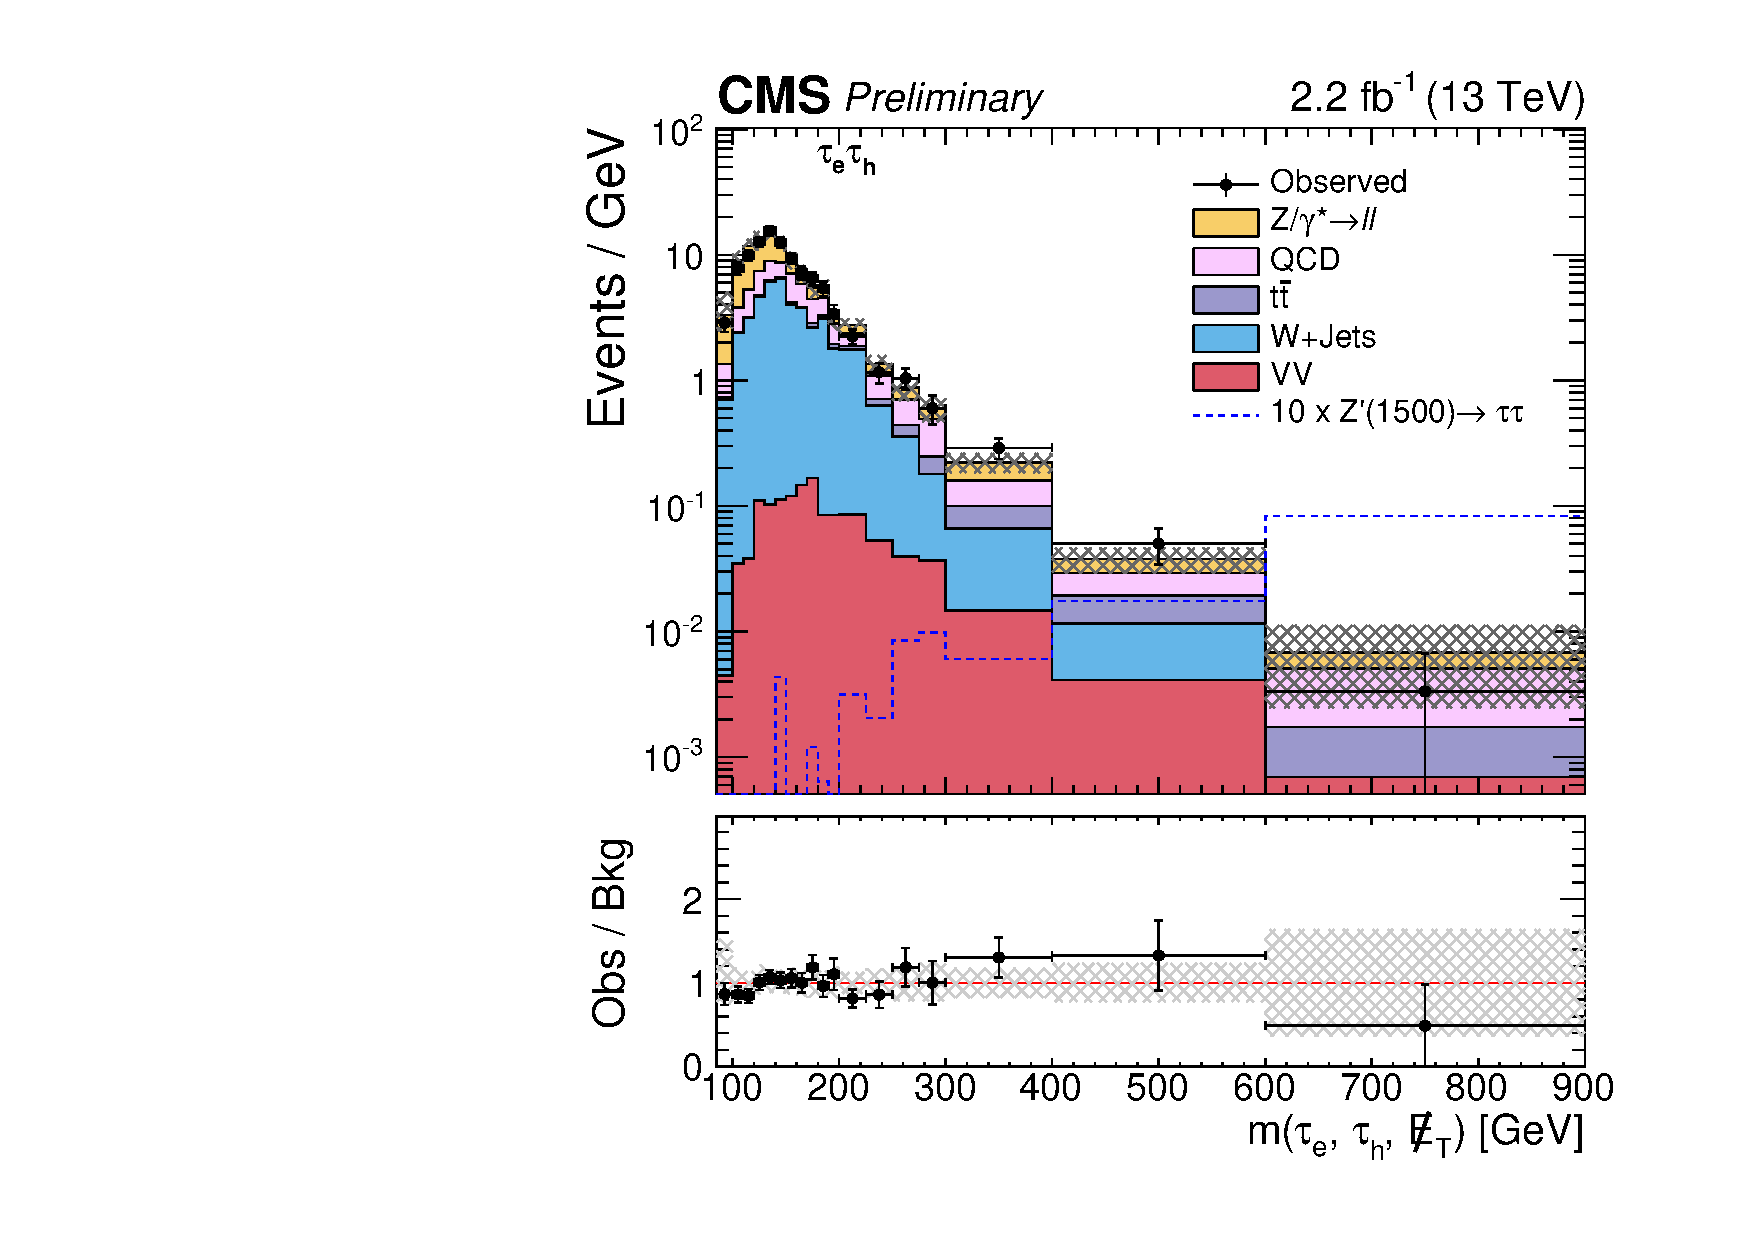
\includegraphics[width=0.4\textwidth]{figures/bkgTemplate_ZPrime1500_et.pdf}
   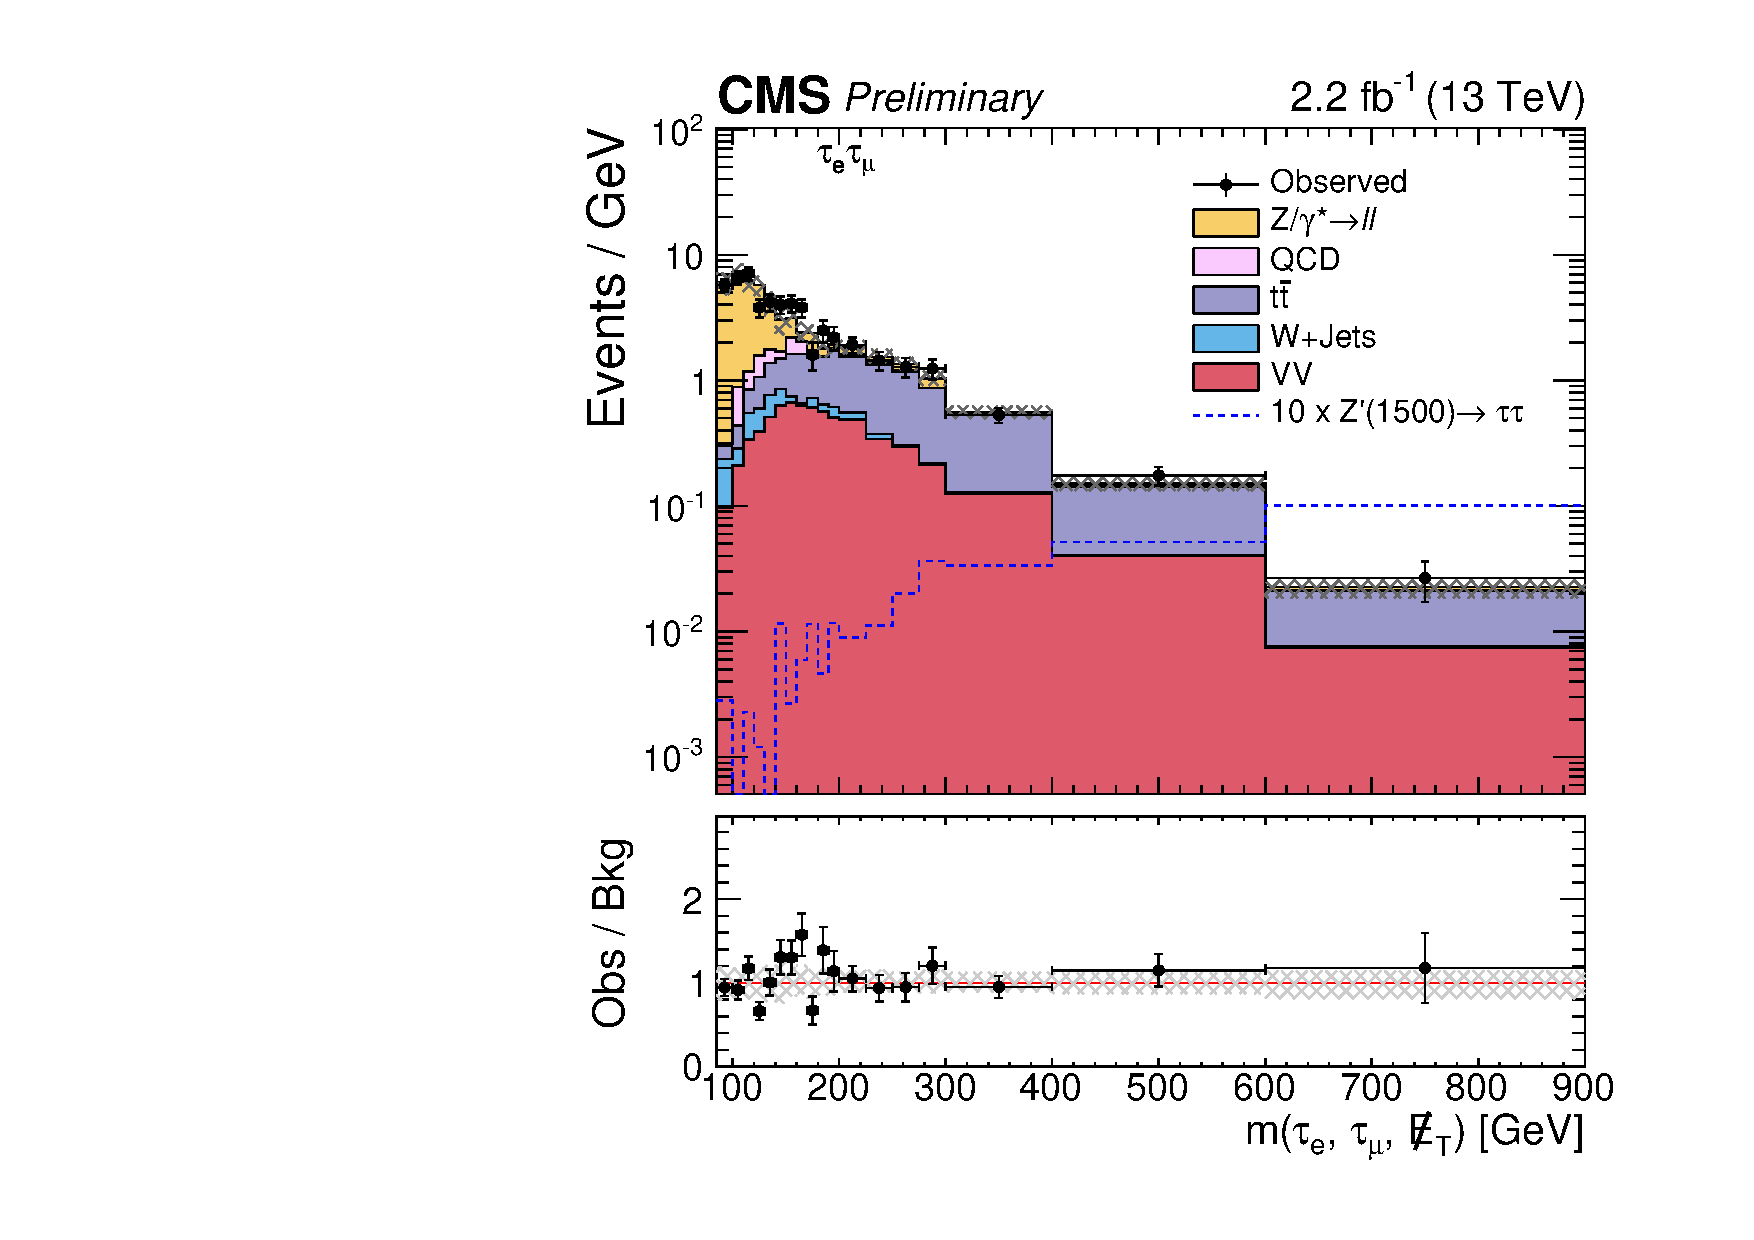
\includegraphics[width=0.4\textwidth]{figures/bkgTemplate_ZPrime1500_em.pdf}
  \caption{ Top Left: $m(\mu,\tau_{h},\MET)$ distribution in the signal region, in log scale.  Top Right: $m(\tau_{h},\tau_{h},\MET)$ distribution in 
the signal region, in log scale.  Bottom Left: $m(e,\tau_{h},\MET)$ distribution in the signal region, in log scale.  Bottom Right: $m(e,\mu,\MET)$ 
distribution in the signal region, in log scale.}
    \label{fig:SignalRegionPlot_a}
\end{figure}

\begin{table}[ht]
\begin{center}
  \caption{Event summary table after signal region selection\label{tab:summaryTable}}
  \begin{tabular}{| l | c | c | c | c |}
  \hline
       Process          & \ditauh             & \mutau                 & \etau                 & \emu            \\ \hline
       Z' (500)         & 307.4 $\pm$ 35.3  & 502.3 $\pm$ 57.7      & 197.6 $\pm$ 22.7      & 218.6 $\pm$ 27.3  \\   
       Z' (1000)        & 34.6 $\pm$ 2.6    & 40.8 $\pm$ 3.1        & 14.7 $\pm$ 1.1        & 19.0 $\pm$ 1.5        \\   
       Z' (1500)        & 6.6 $\pm$ 0.3     & 7.2 $\pm$ 0.3         & 2.3 $\pm$ 0.1         & 3.6 $\pm$ 0.2      \\   
       Z' (2000)        & 1.6 $\pm$ 0.07    & 1.8 $\pm$ 0.08        & 0.59 $\pm$ 0.03       & 0.91 $\pm$ 0.04        \\   
       Z' (2500)        & 0.55 $\pm$ 0.02   & 0.60 $\pm$ 0.02       & 0.19 $\pm$ 0.01       & 0.30 $\pm$ 0.01       \\   
       Z' (3000)        & 0.13 $\pm$ 0.01   & 0.14 $\pm$ 0.01       & 0.04 $\pm$ 0.00       & 0.07 $\pm$ 0.00   \\   
       Drell-Yan        & 8.4 $\pm$ 3.1     & 882.4 $\pm$ 127.0     & 375.1 $\pm$ 117.6     & 321.2 $\pm$ 99.2 \\
       W+jets           & 0.1 $\pm$ 0.1     & 916.2 $\pm$ 96.1      & 545.8 $\pm$ 85.6      & 18.9 $\pm$ 11.4 \\
       Diboson          & 0.5 $\pm$ 0.5     & 29.2 $\pm$ 7.4        & 18.0 $\pm$ 4.4        & 108.3 $\pm$ 17.4 \\
       $t\bar{t}$       & --                & 26.1 $\pm$ 6.7        & 26.1 $\pm$ 7.5        & 222.8 $\pm$ 44.8 \\
       Multijet         & 48.7 $\pm$ 13.0   & 121.8 $\pm$ 83.5      & 116.7 $\pm$ 71.5      & 31.9 $\pm$ 24.3 \\
       Observation      & 55                & 1807                  & 1113                  & 728        \\
  \hline
  \end{tabular}
\end{center}
\end{table}


%\begin{figure}[tbh!]
%  \centering
%    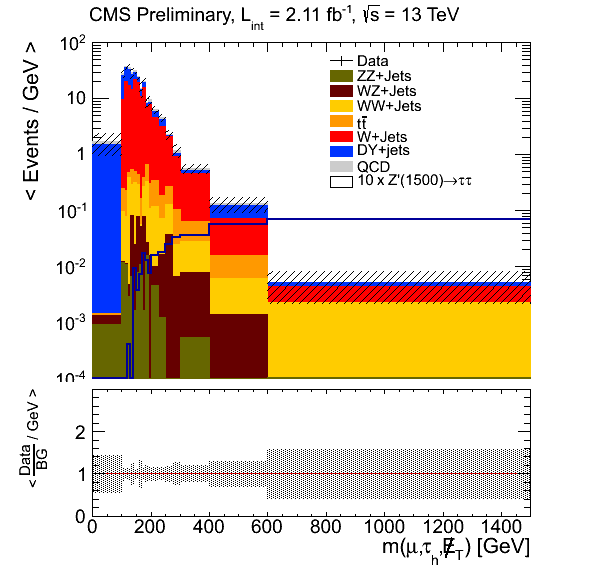
\includegraphics[width=0.4\textwidth]{figures/SRplot_NoData.png}
%    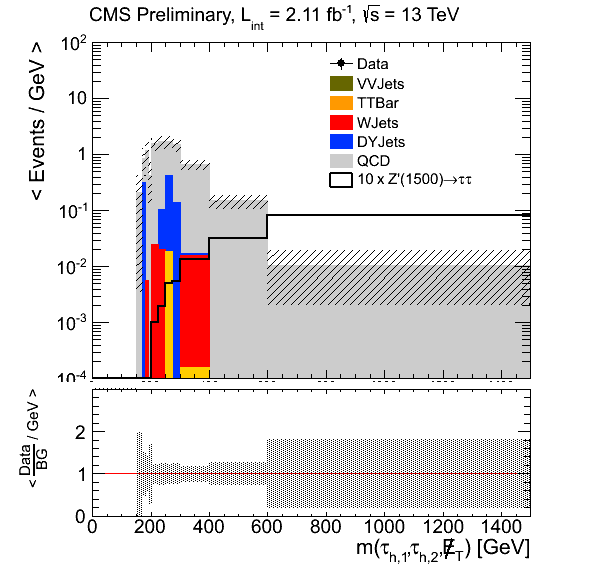
\includegraphics[width=0.4\textwidth]{figures/SRplot_diTauHad_NoData.png} \\
%    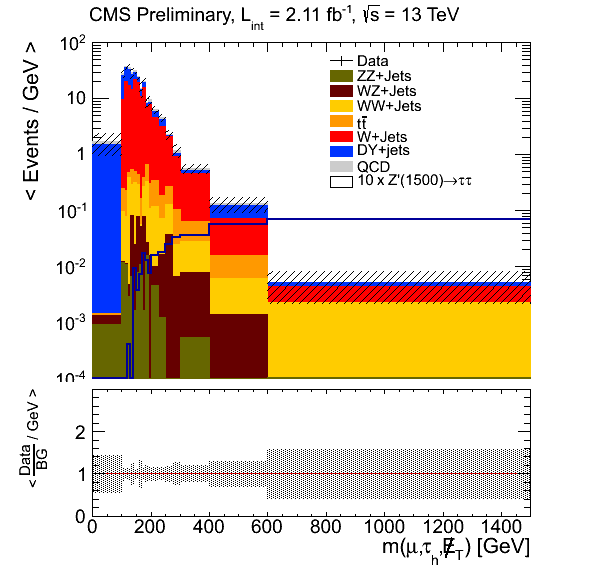
\includegraphics[width=0.4\textwidth]{figures/SRplot_NoData.png}
%    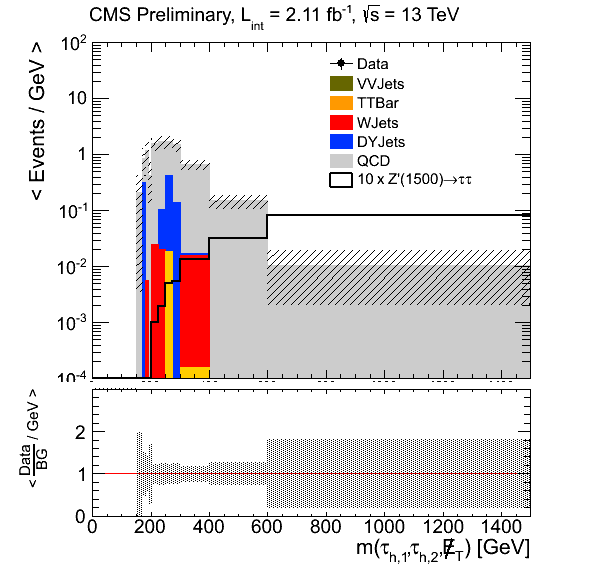
\includegraphics[width=0.4\textwidth]{figures/SRplot_diTauHad_NoData.png} 
%  \caption{ Top Left: $m(\mu,\tau_{h},\MET)$ distribution in the signal region, in normal scale.  Top Right: $m(\tau_{h},\tau_{h},\MET)$ distribution in 
%the signal region, in normal scale.  Bottom Left: $m(e,\tau_{h},\MET)$ distribution in the signal region, in normal scale.  Bottom Right: $m(e,\mu,\MET)$ 
%distribution in the signal region, in normal scale.}
%    \label{fig:SignalRegionPlot_b}
%\end{figure}

\begin{figure}[tbh!]
  \centering
  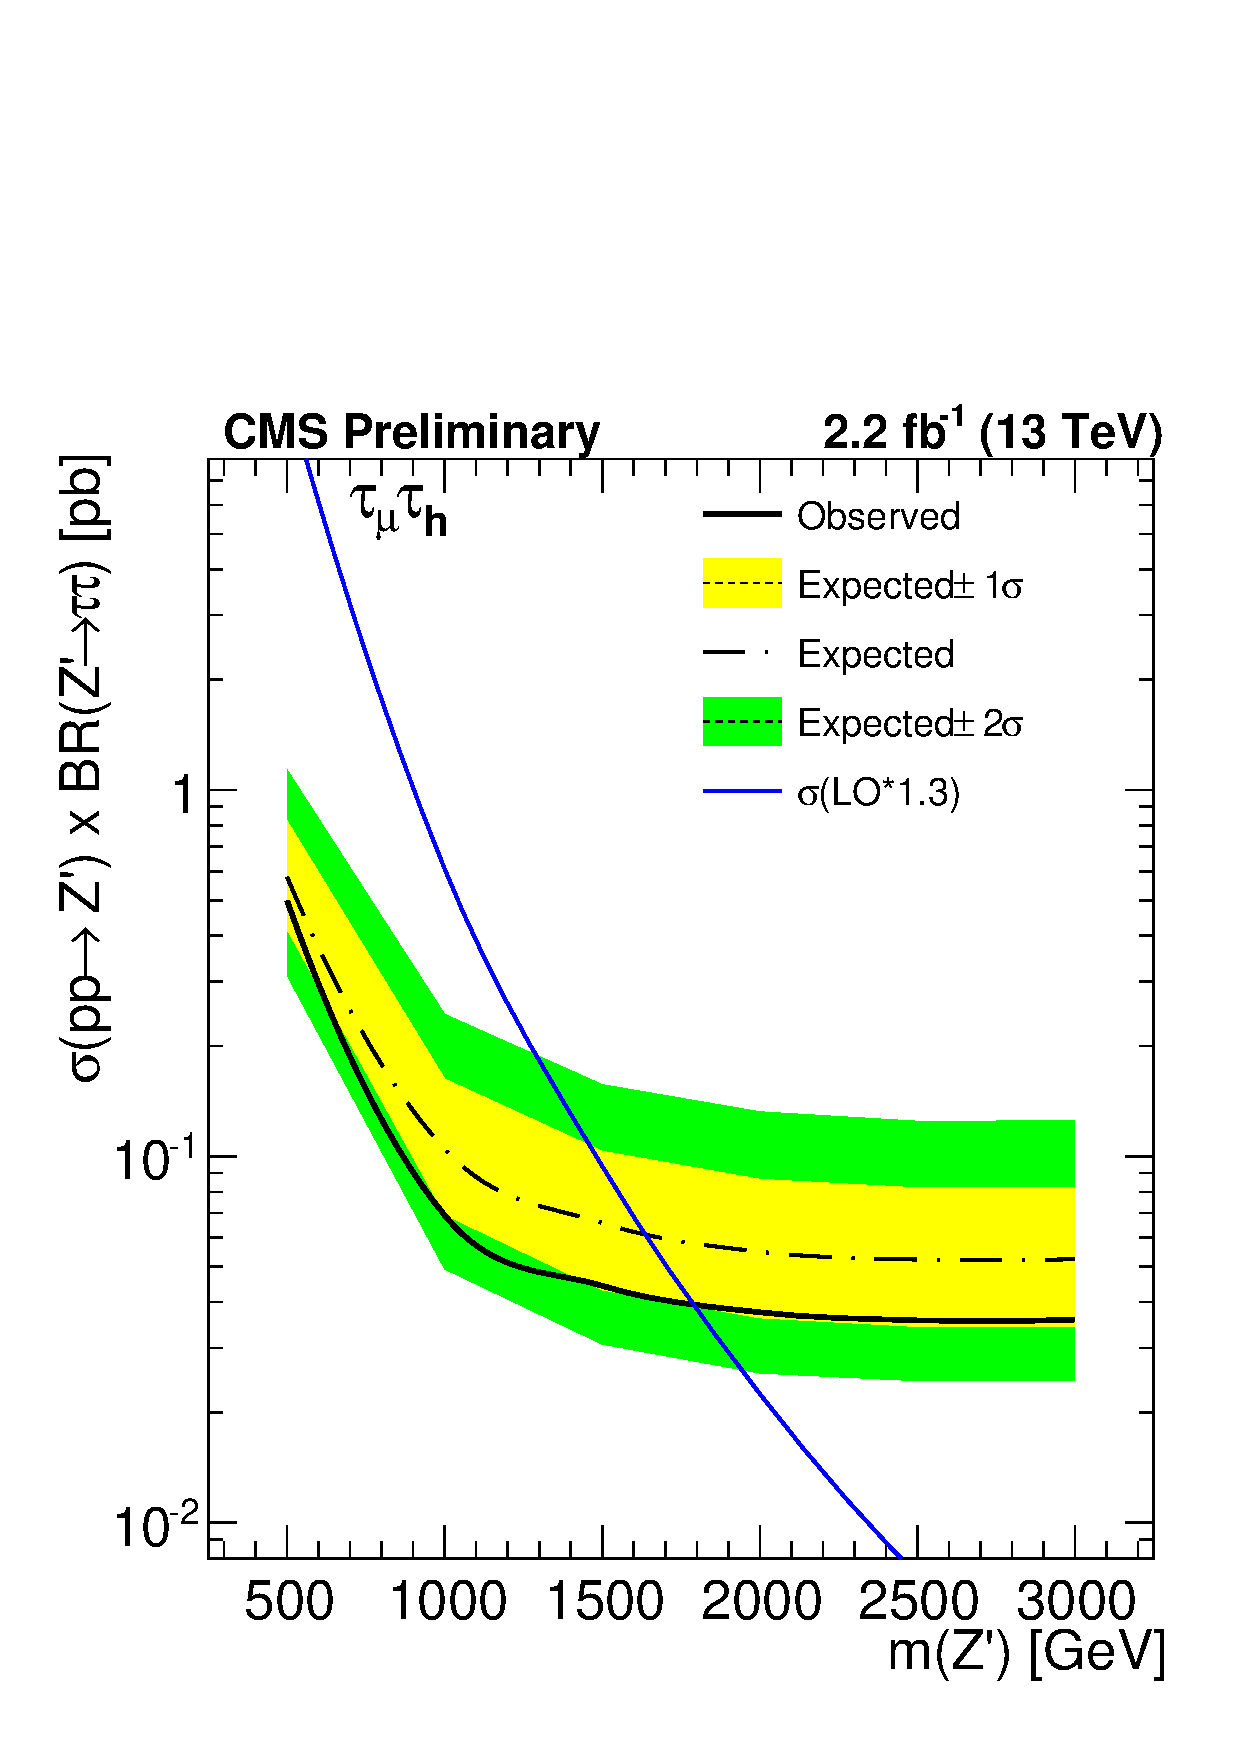
\includegraphics[width=0.4\textwidth]{figures/limits/Limit_muTau.pdf}
  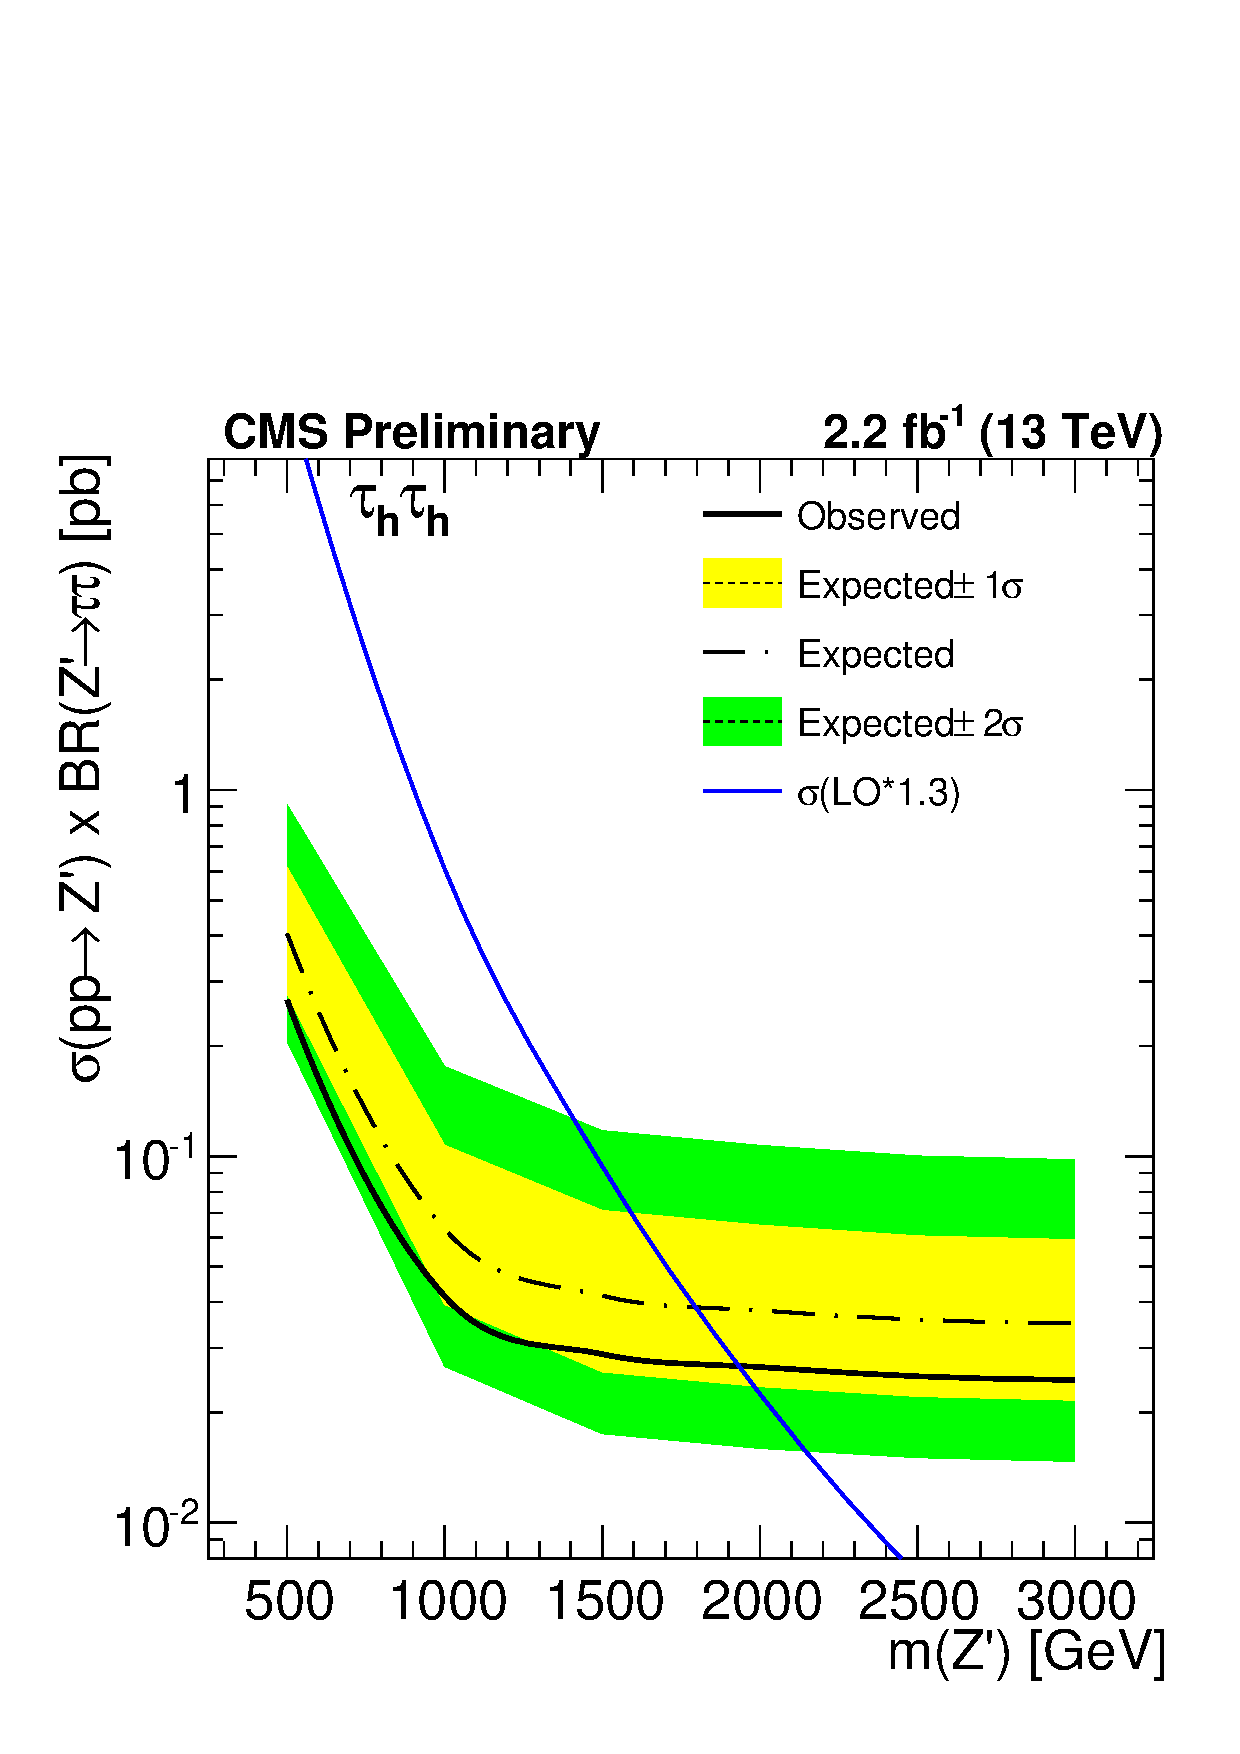
\includegraphics[width=0.4\textwidth]{figures/limits/Limit_TauTau}\\
  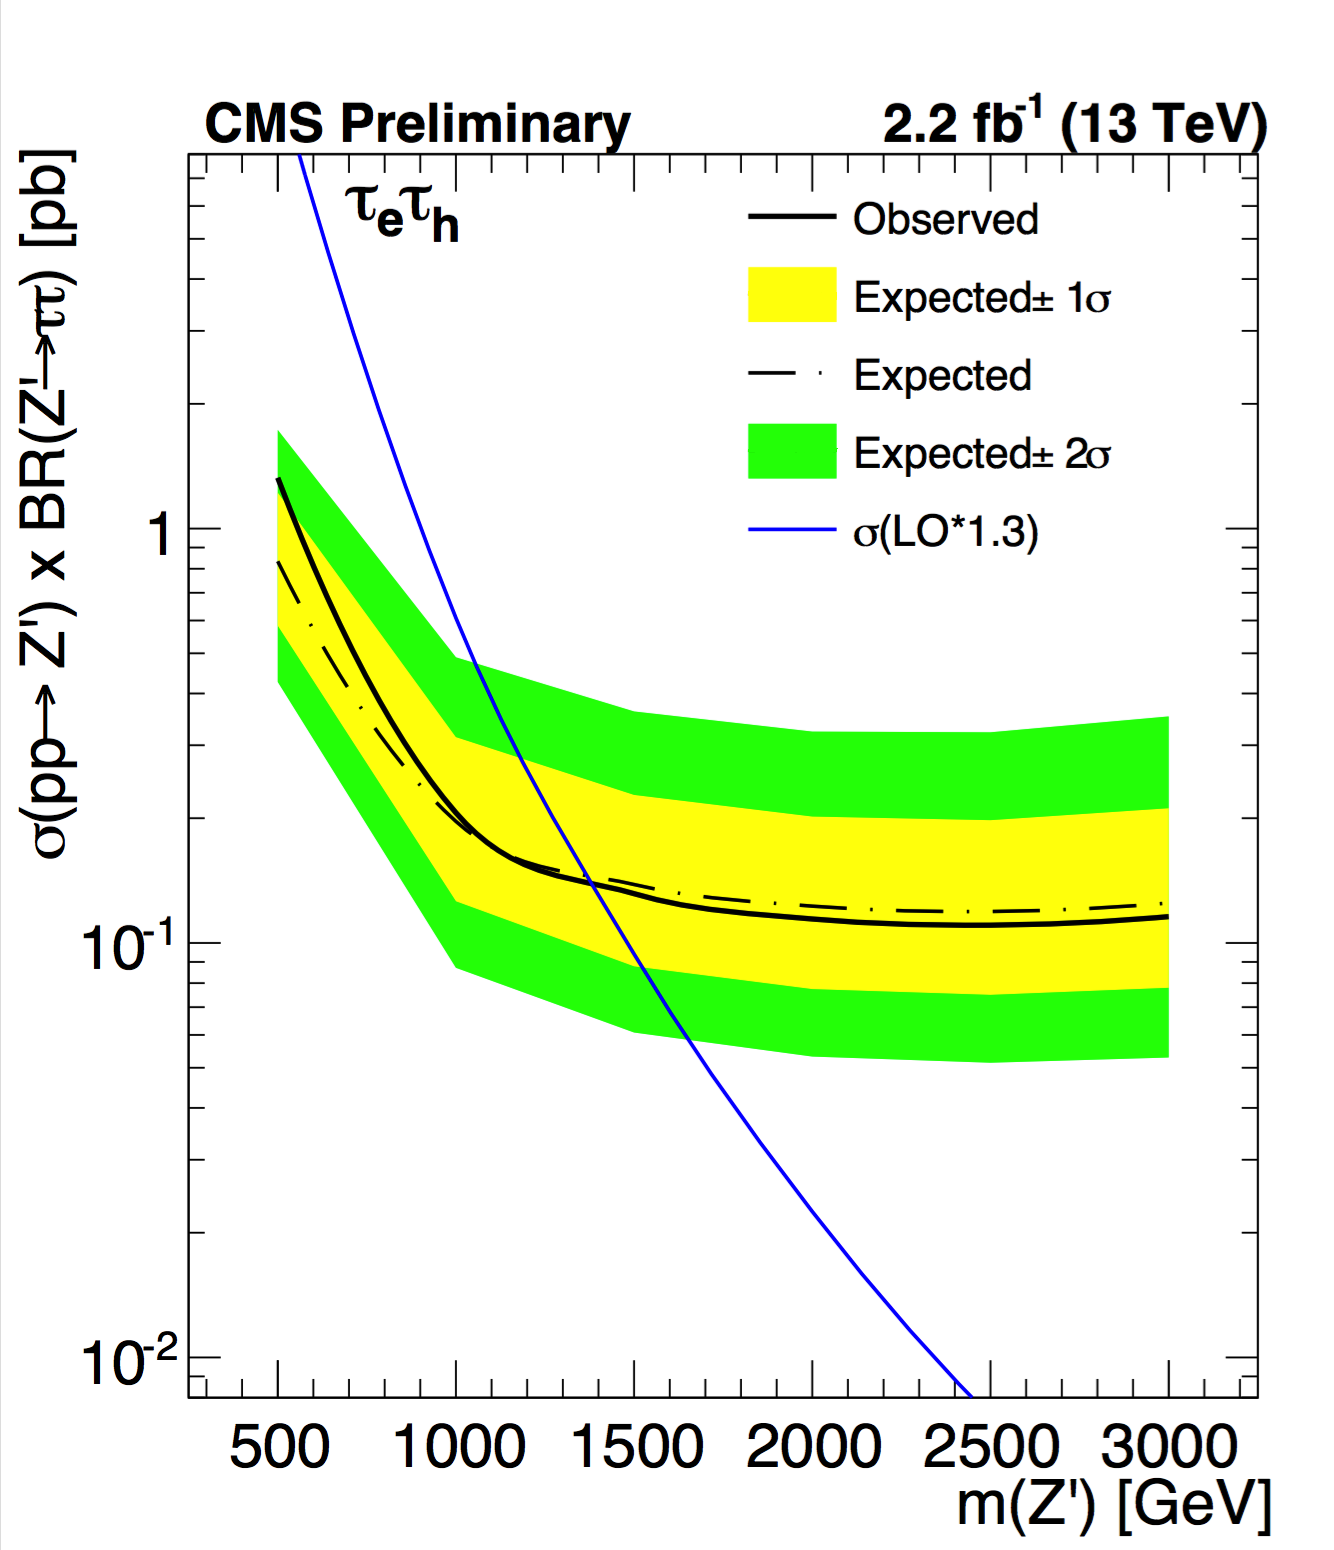
\includegraphics[width=0.4\textwidth]{figures/limits/Limit_eTau}
  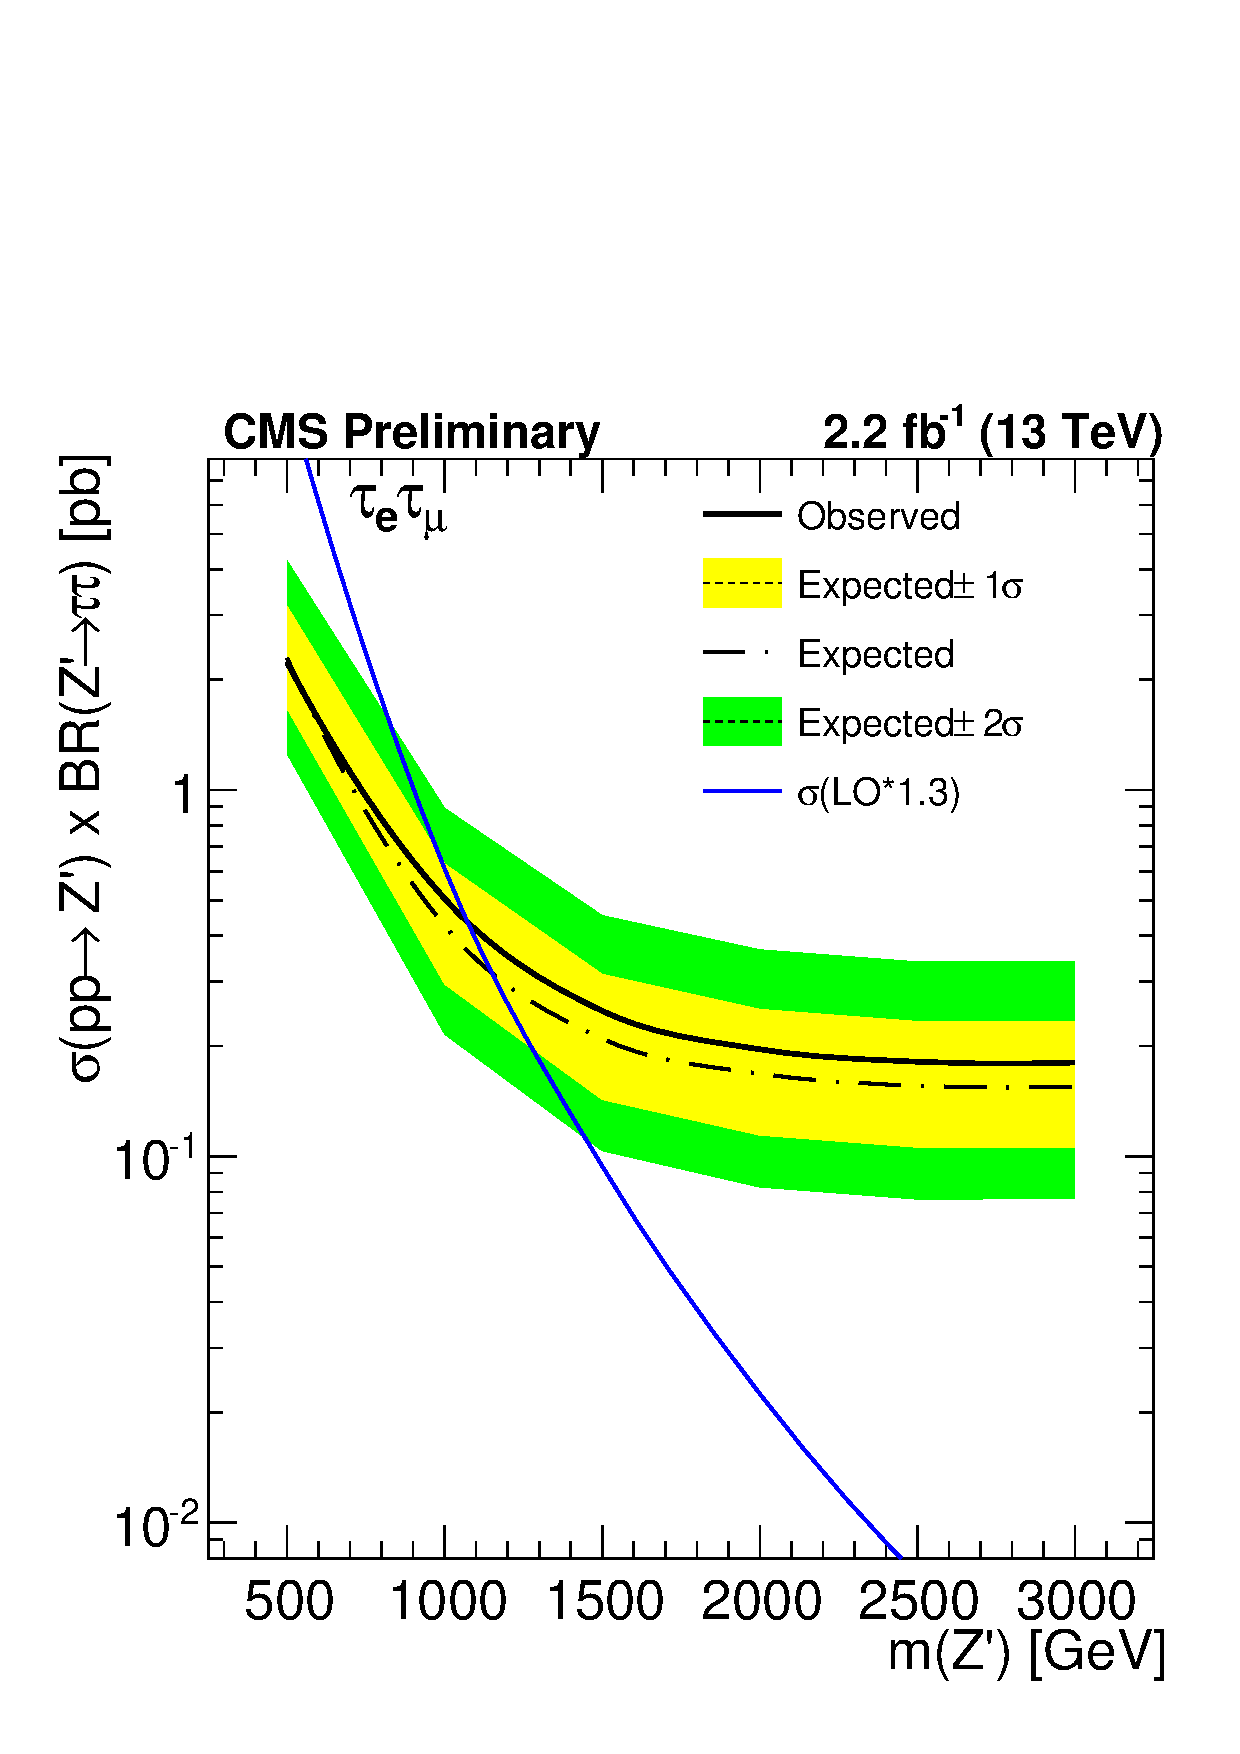
\includegraphics[width=0.4\textwidth]{figures/limits/Limit_eMu.pdf}
  \caption{Expected and observed limits for the $\tau_{\mu}\tau_{h}$, $\tau_{h}\tau_{h}$, $\tau_{e}\tau_{h}$, $\tau_{e}\tau_{\mu}$ channels. A k factor of 1.3 has been used to scale the leading order (LO) signal cross-section.} 
    \label{fig:Limits}
\end{figure}

\begin{figure}[tbh!]
  \centering
  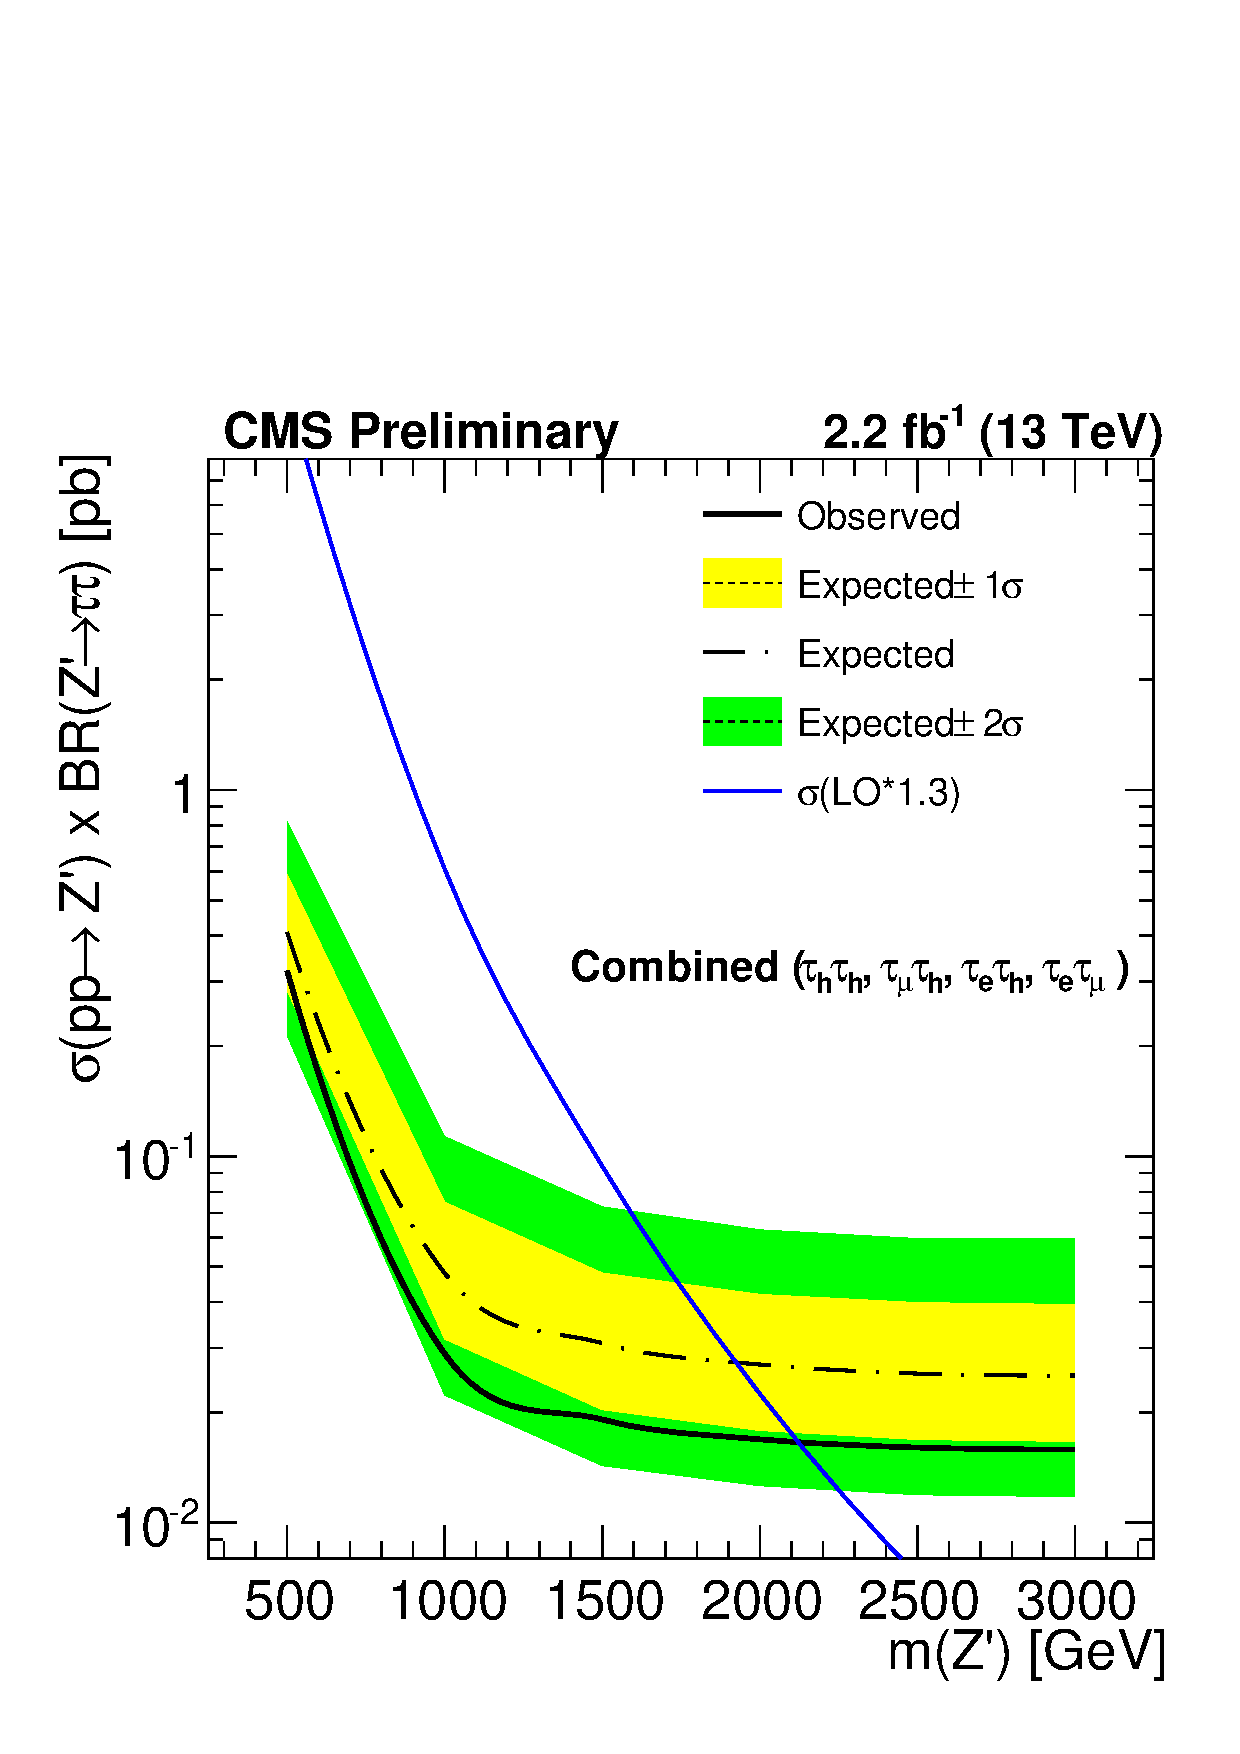
\includegraphics[width=0.6\textwidth]{figures/limits/CombinedLimit}  \caption{Combined expected limit for the $\tau_{\mu}\tau_{h}$, $\tau_{h}\tau_{h}$, $\tau_{e}\tau_{h}$, $\tau_{e}\tau_{\mu}$ channels.}
  \caption{Combined expected limit for the $\tau_{\mu}\tau_{h}$, $\tau_{h}\tau_{h}$, $\tau_{e}\tau_{h}$, $\tau_{e}\tau_{\mu}$ channels. A k factor of 1.3 has been used to scale the leading order (LO) signal cross-section.}
  \label{fig:CombinedLimits}
\end{figure}



\section{8 TeV Results}

The search for $Z^{\prime}\to\tau\tau$ events was also carried out during the 2012 run of the LHC, when the center-of-mass collision energy was lower at $\sqrt{s} = 8$ TeV. 19.7 fb$^{-1}$ of collision data were collected during this run. Due to poor performance of the Tau POG recommended hadronic tau identification and reconstruction algorithms, the only channel which was studied to completion was the \emu channel. As the analysis strategy, trigger studies, and background estimation techniques were nearly identical to those presented for the \emu channel at $\sqrt{s} = 13$ TeV, only the results of the 8 TeV \emu analysis are shown here.

Figure \ref{fig:8TeV_SR} and Figure \ref{fig:8TeV_BGRates} show the unblinded signal region and background rates after all backgrounds are estimated. Data agrees with SM expectation, so limits are set on the $Z^{\prime}_{SSM}$ visible mass and the $E_6$-inspired $Z^{\prime}_{\psi}$ visible mass.

\begin{figure}[tbh!]
\centering
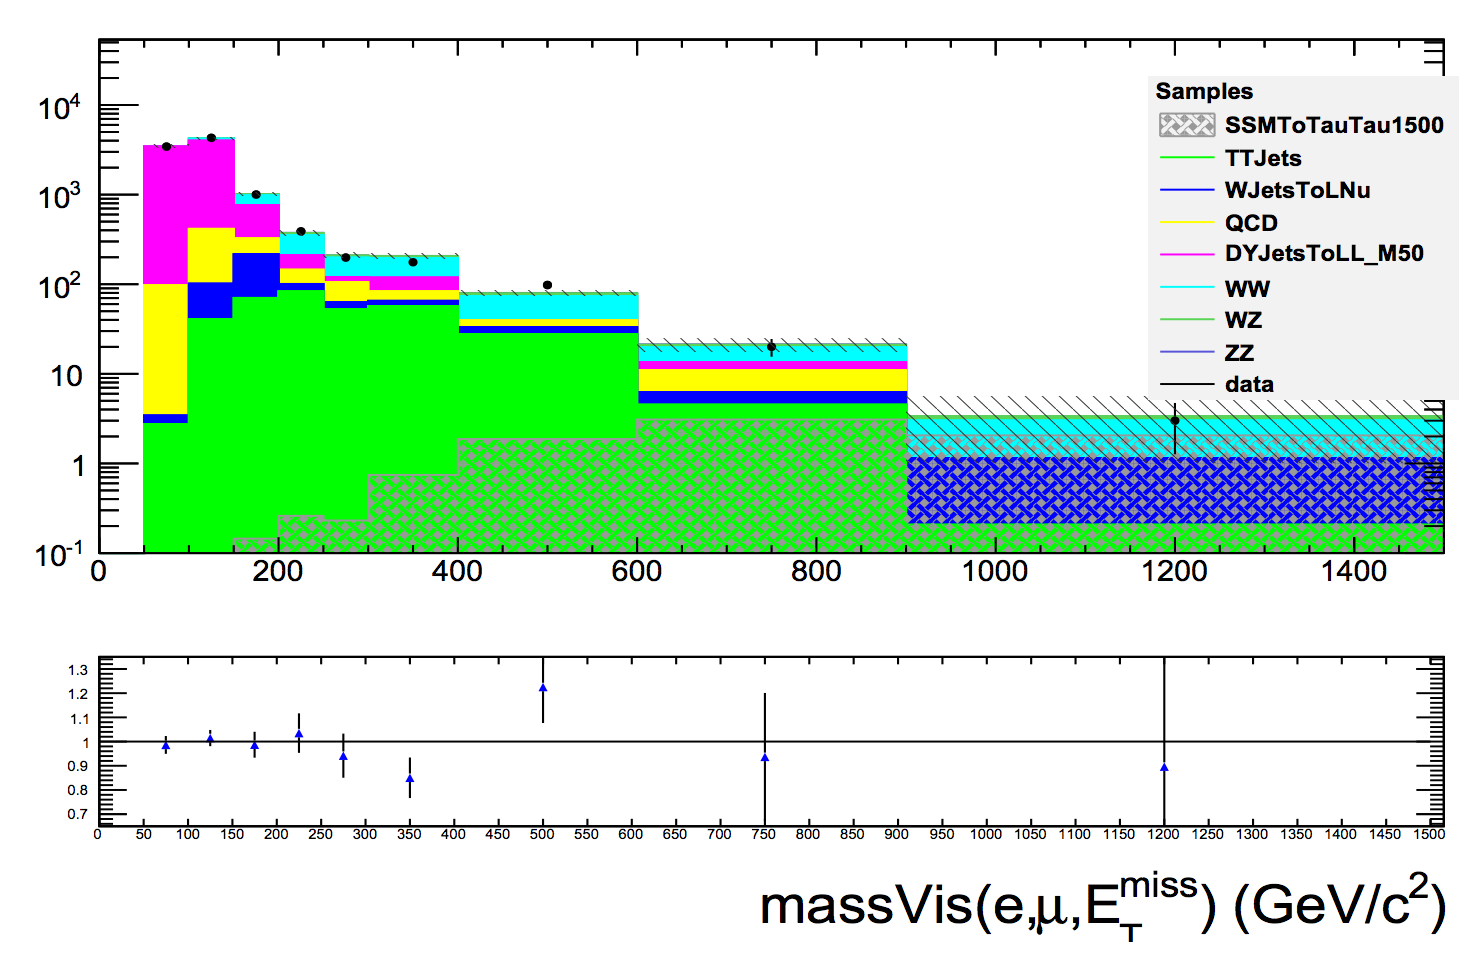
\includegraphics[width=0.6\textwidth]{figures/8TeV_SR.png}
\caption{$m(e,\tau_{h},\MET)$ distribution for SR in 8TeV search. A 1.5TeV $Z^{\prime}_{SSM}$ sample is also included.}
\label{fig:8TeV_SR}
\end{figure}

\begin{figure}[tbh!]
\centering
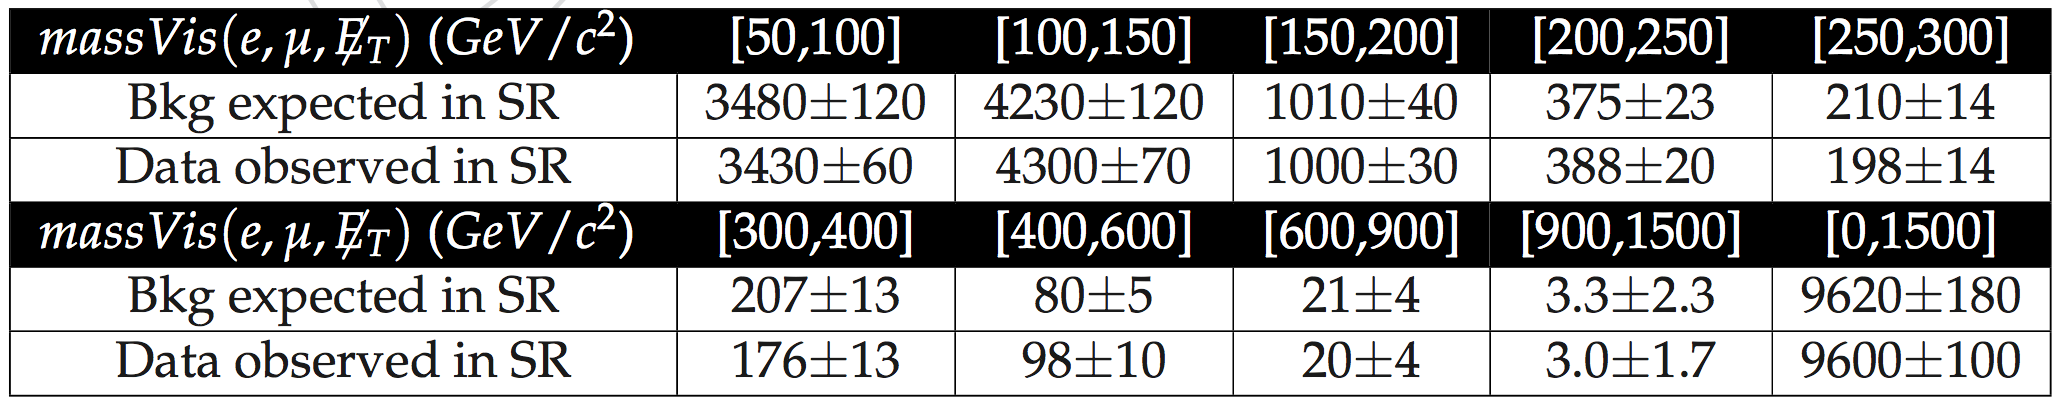
\includegraphics[width=0.6\textwidth]{figures/8TeV_BGRates.png}
\caption{Expected background rates compared to observed rates in bins of $m(e,\tau_{h},\MET)$. Uncertainties are statistical in each bin.}
\label{fig:8TeV_BGRates}
\end{figure}

Figure \ref{fig:8TeV_SignalRates} shows the predicted rates in the SR of several $Z^{\prime}_{SSM}$ signal mass points considered in this analysis.

\begin{figure}[tbh!]
\centering
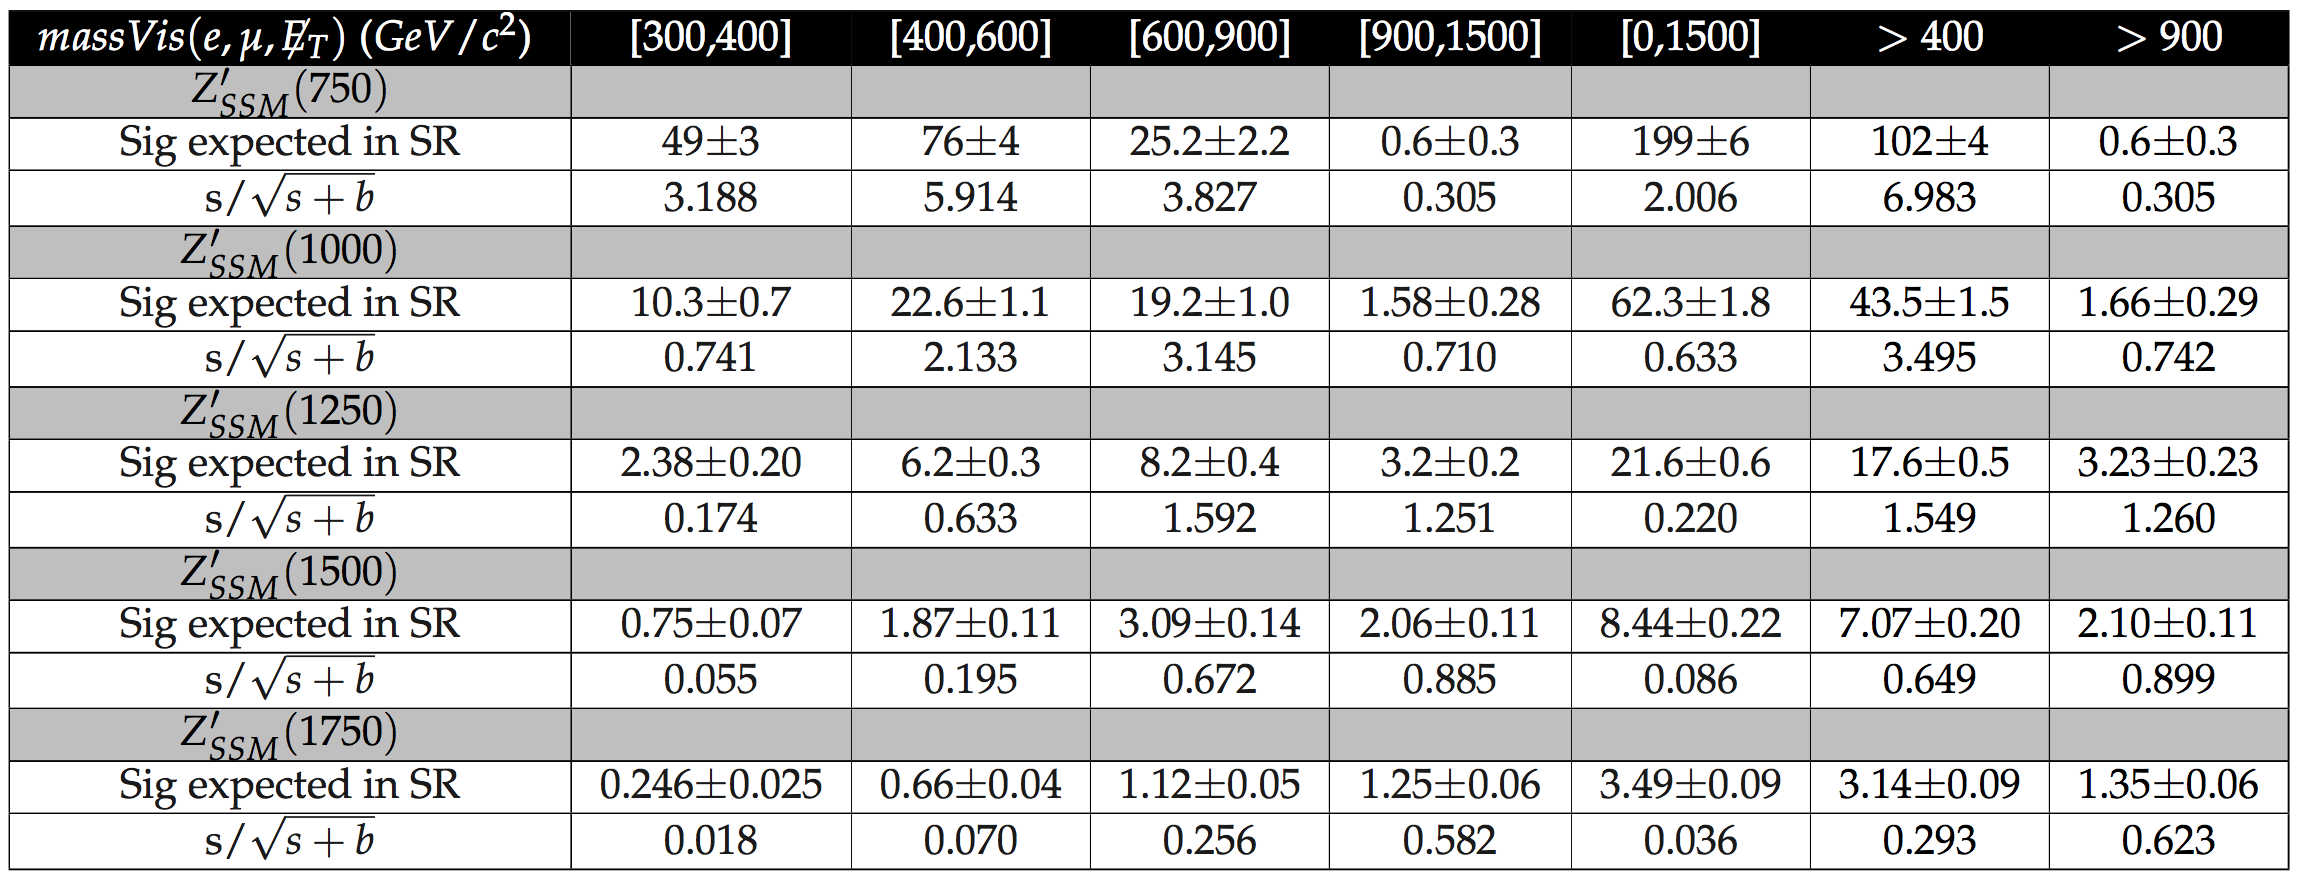
\includegraphics[width=0.6\textwidth]{figures/8TeV_SignalRates.png}
\caption{Expected signal rates and associated significances in bins of $m(e,\tau_{h},\MET)$. }
\label{fig:8TeV_SignalRates}
\end{figure}

Finally, the limit on a $Z^{\prime}_{SSM}$ decaying to two taus are given in Figure \ref{fig:8TeV_Limit}. Upper limits are placed on $\sigma\left(pp\to Z^{\prime}\right)\times BR\left(Z^{\prime}\to\tau\tau\right)$ as a function of mass. The limit is set as the point at which the experimental value of $\sigma\left(pp\to Z^{\prime}\right)\times BR\left(Z^{\prime}\to\tau\tau\right)$ exceeds the theoretical value. Below this point, we exclude the existence of $Z^{\prime}$-like particles decaying to tau pairs. Figure \ref{fig:8TeV_Limits} shows that we exclude the $Z^{\prime}_{SSM}$ below a mass of 1300 GeV/c$^2$, and that we exclude the $Z^{\prime}_{\psi}$ below a mass of 810 GeV/c$^2$.

\begin{figure}[tbh!]
\centering
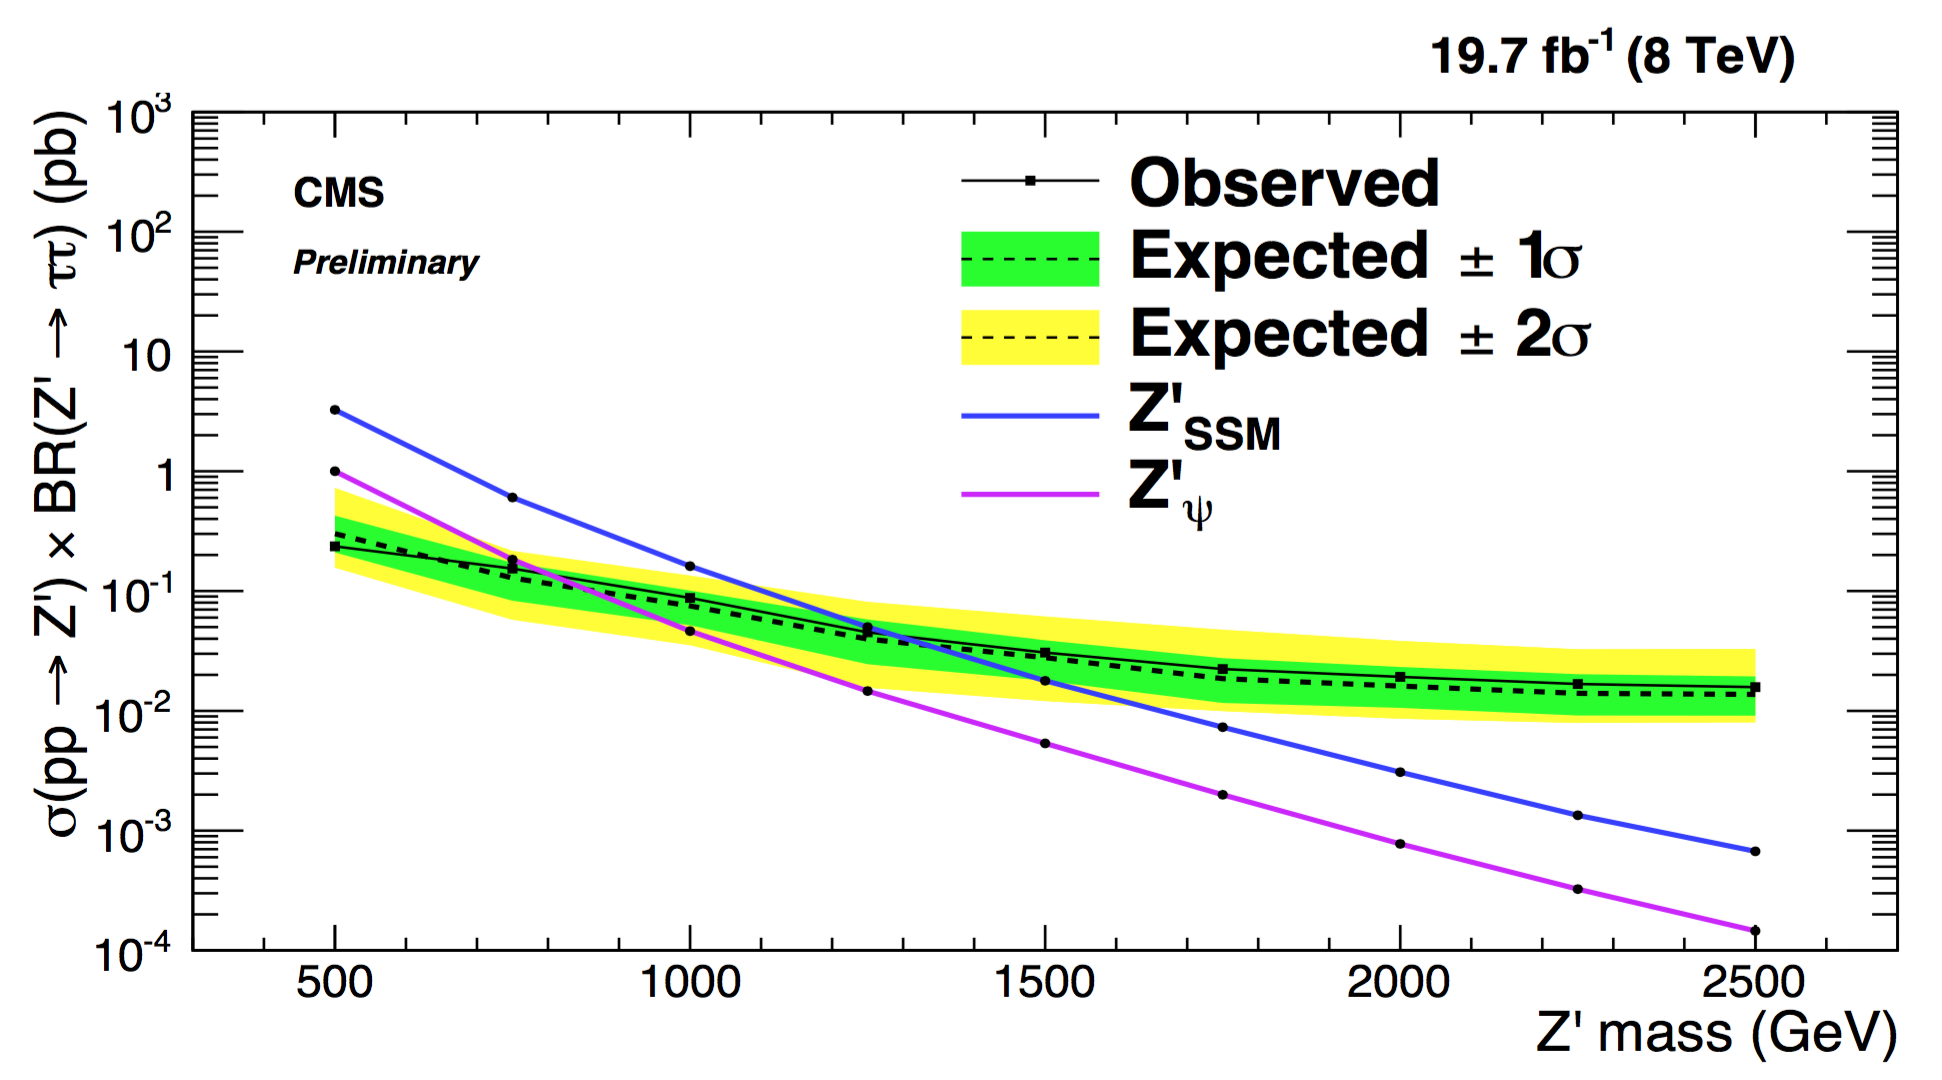
\includegraphics[width=0.6\textwidth]{figures/8TeV_Limits.png}
\caption{95\% CL upper limit on $\sigma\left(pp\to Z^{\prime}\right)\times BR\left(Z^{\prime}\to\tau\tau\right)$ 
as a function of $Z^{\prime}$ mass. The color bands on the expected limits represent one standard deviation (green) and two standard deviations (yellow).}
\label{fig:8TeV_Limits}
\end{figure}
